\documentclass{standalone}
\usepackage{tikz}
\usetikzlibrary{patterns, positioning}


\begin{document}
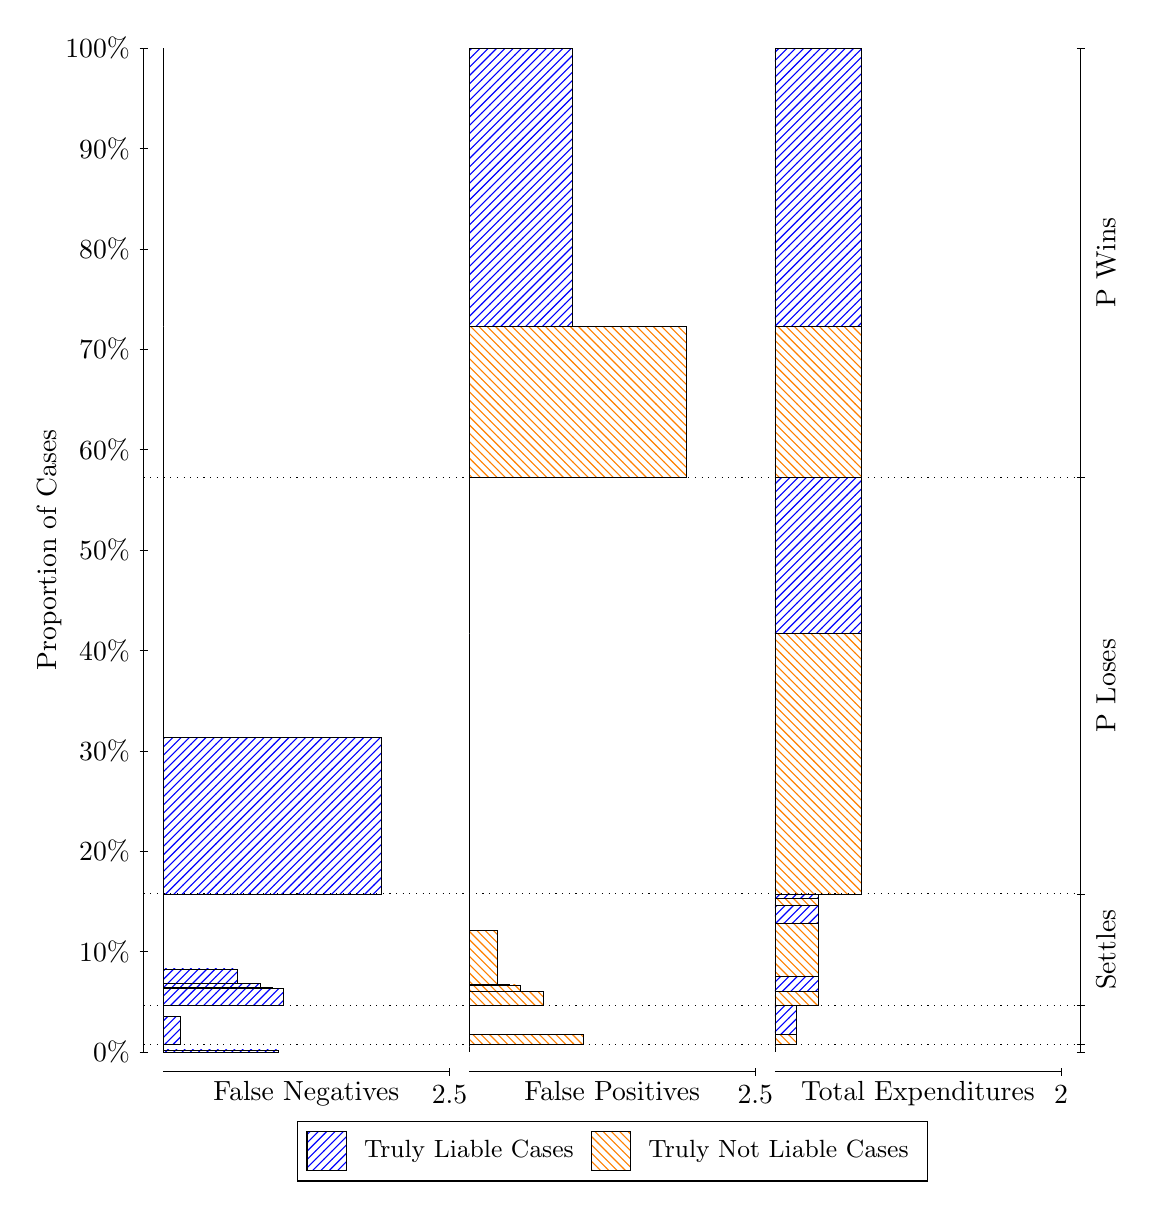
\begin{tikzpicture}
\draw[black, very thin] (1.5,1.75) -- (1.5,14.5);
\node[rotate=90, text=black, anchor=center] at (0.3, 8.125) {Proportion of Cases};
\draw[black, very thin] (1.45,1.75) -- (1.55,1.75);
\node[text=black, anchor=east] at (1.45, 1.75) {0\%};
\draw[black, very thin] (1.45,3.025) -- (1.55,3.025);
\node[text=black, anchor=east] at (1.45, 3.025) {10\%};
\draw[black, very thin] (1.45,4.3) -- (1.55,4.3);
\node[text=black, anchor=east] at (1.45, 4.3) {20\%};
\draw[black, very thin] (1.45,5.575) -- (1.55,5.575);
\node[text=black, anchor=east] at (1.45, 5.575) {30\%};
\draw[black, very thin] (1.45,6.85) -- (1.55,6.85);
\node[text=black, anchor=east] at (1.45, 6.85) {40\%};
\draw[black, very thin] (1.45,8.125) -- (1.55,8.125);
\node[text=black, anchor=east] at (1.45, 8.125) {50\%};
\draw[black, very thin] (1.45,9.4) -- (1.55,9.4);
\node[text=black, anchor=east] at (1.45, 9.4) {60\%};
\draw[black, very thin] (1.45,10.675) -- (1.55,10.675);
\node[text=black, anchor=east] at (1.45, 10.675) {70\%};
\draw[black, very thin] (1.45,11.95) -- (1.55,11.95);
\node[text=black, anchor=east] at (1.45, 11.95) {80\%};
\draw[black, very thin] (1.45,13.225) -- (1.55,13.225);
\node[text=black, anchor=east] at (1.45, 13.225) {90\%};
\draw[black, very thin] (1.45,14.5) -- (1.55,14.5);
\node[text=black, anchor=east] at (1.45, 14.5) {100\%};

\draw[black, very thin] (13.4,1.75) -- (13.4,14.5);
\draw[black, very thin] (13.35,1.75) -- (13.45,1.75);
\node[anchor=west] at (13.35, 1.75) {};
\draw[black, very thin] (13.35,1.8419) -- (13.45,1.8419);
\node[anchor=west] at (13.35, 1.8419) {};
\draw[black, very thin] (13.35,2.3398) -- (13.45,2.3398);
\node[anchor=west] at (13.35, 2.3398) {};
\draw[black, very thin] (13.35,3.758) -- (13.45,3.758);
\node[anchor=west] at (13.35, 3.758) {};
\draw[black, very thin] (13.35,9.0514) -- (13.45,9.0514);
\node[anchor=west] at (13.35, 9.0514) {};
\draw[black, very thin] (13.35,14.5) -- (13.45,14.5);
\node[anchor=west] at (13.35, 14.5) {};

\draw[black, very thin, pattern color=blue, pattern=north east lines] (1.75,1.75) rectangle (3.2033,1.7752);
\draw[black, very thin, pattern color=orange, pattern=north west lines] (1.75,1.7752) rectangle (1.75,1.8419);
\draw[black, very thin, pattern color=blue, pattern=north east lines] (1.75,1.8419) rectangle (1.968,2.2037);
\draw[black, very thin, pattern color=orange, pattern=north west lines] (1.75,2.2037) rectangle (1.75,2.3398);
\draw[black, very thin, pattern color=blue, pattern=north east lines] (1.75,2.3398) rectangle (3.276,2.5622);
\draw[black, very thin, pattern color=blue, pattern=north east lines] (1.75,2.5622) rectangle (3.1307,2.5654);
\draw[black, very thin, pattern color=blue, pattern=north east lines] (1.75,2.5654) rectangle (2.9853,2.6228);
\draw[black, very thin, pattern color=blue, pattern=north east lines] (1.75,2.6228) rectangle (2.6947,2.805);
\draw[black, very thin, pattern color=orange, pattern=north west lines] (1.75,2.805) rectangle (1.75,3.758);
\draw[black, very thin, pattern color=blue, pattern=north east lines] (1.75,3.758) rectangle (4.5113,5.7451);
\draw[black, very thin, pattern color=orange, pattern=north west lines] (1.75,5.7451) rectangle (1.75,9.0514);
\draw[black, very thin, pattern color=orange, pattern=north west lines] (1.75,9.0514) rectangle (1.75,10.964);
\draw[black, very thin, pattern color=blue, pattern=north east lines] (1.75,10.964) rectangle (1.75,14.5);
\draw[black, very thin, pattern color=orange, pattern=north west lines] (5.6333,1.75) rectangle (5.6333,1.8167);
\draw[black, very thin, pattern color=blue, pattern=north east lines] (5.6333,1.8167) rectangle (5.6333,1.8419);
\draw[black, very thin, pattern color=orange, pattern=north west lines] (5.6333,1.8419) rectangle (7.0867,1.9781);
\draw[black, very thin, pattern color=blue, pattern=north east lines] (5.6333,1.9781) rectangle (5.6333,2.3398);
\draw[black, very thin, pattern color=orange, pattern=north west lines] (5.6333,2.3398) rectangle (6.578,2.5229);
\draw[black, very thin, pattern color=orange, pattern=north west lines] (5.6333,2.5229) rectangle (6.2873,2.6011);
\draw[black, very thin, pattern color=orange, pattern=north west lines] (5.6333,2.6011) rectangle (6.142,2.609);
\draw[black, very thin, pattern color=orange, pattern=north west lines] (5.6333,2.609) rectangle (5.9967,3.2928);
\draw[black, very thin, pattern color=blue, pattern=north east lines] (5.6333,3.2928) rectangle (5.6333,3.758);
\draw[black, very thin, pattern color=orange, pattern=north west lines] (5.6333,3.758) rectangle (5.6333,7.0642);
\draw[black, very thin, pattern color=blue, pattern=north east lines] (5.6333,7.0642) rectangle (5.6333,9.0514);
\draw[black, very thin, pattern color=orange, pattern=north west lines] (5.6333,9.0514) rectangle (8.3947,10.964);
\draw[black, very thin, pattern color=blue, pattern=north east lines] (5.6333,10.964) rectangle (6.9413,14.5);
\draw[black, very thin, pattern color=orange, pattern=north west lines] (9.5167,1.75) rectangle (9.5167,1.8167);
\draw[black, very thin, pattern color=blue, pattern=north east lines] (9.5167,1.8167) rectangle (9.5167,1.8419);
\draw[black, very thin, pattern color=orange, pattern=north west lines] (9.5167,1.8419) rectangle (9.7892,1.9781);
\draw[black, very thin, pattern color=blue, pattern=north east lines] (9.5167,1.9781) rectangle (9.7892,2.3398);
\draw[black, very thin, pattern color=orange, pattern=north west lines] (9.5167,2.3398) rectangle (10.062,2.5229);
\draw[black, very thin, pattern color=blue, pattern=north east lines] (9.5167,2.5229) rectangle (10.062,2.7051);
\draw[black, very thin, pattern color=orange, pattern=north west lines] (9.5167,2.7051) rectangle (10.062,3.3889);
\draw[black, very thin, pattern color=blue, pattern=north east lines] (9.5167,3.3889) rectangle (10.062,3.6113);
\draw[black, very thin, pattern color=orange, pattern=north west lines] (9.5167,3.6113) rectangle (10.062,3.6974);
\draw[black, very thin, pattern color=blue, pattern=north east lines] (9.5167,3.6974) rectangle (10.062,3.758);
\draw[black, very thin, pattern color=orange, pattern=north west lines] (9.5167,3.758) rectangle (10.607,7.0642);
\draw[black, very thin, pattern color=blue, pattern=north east lines] (9.5167,7.0642) rectangle (10.607,9.0514);
\draw[black, very thin, pattern color=orange, pattern=north west lines] (9.5167,9.0514) rectangle (10.607,10.964);
\draw[black, very thin, pattern color=blue, pattern=north east lines] (9.5167,10.964) rectangle (10.607,14.5);
\draw[black, dotted] (1.5,1.8419) -- (13.4,1.8419);
\draw[black, dotted] (1.5,2.3398) -- (13.4,2.3398);
\draw[black, dotted] (1.5,3.758) -- (13.4,3.758);
\draw[black, dotted] (1.5,9.0514) -- (13.4,9.0514);
\draw[black, very thin] (1.75,1.5) -- (5.3833,1.5);
\node[text=black, anchor=north] at (3.5667, 1.5) {False Negatives};
\draw[black, very thin] (5.3833,1.45) -- (5.3833,1.55);
\node[text=black, anchor=north] at (5.3833, 1.45) {2.5};

\draw[black, very thin] (5.6333,1.5) -- (9.2667,1.5);
\node[text=black, anchor=north] at (7.45, 1.5) {False Positives};
\draw[black, very thin] (9.2667,1.45) -- (9.2667,1.55);
\node[text=black, anchor=north] at (9.2667, 1.45) {2.5};

\draw[black, very thin] (9.5167,1.5) -- (13.15,1.5);
\node[text=black, anchor=north] at (11.333, 1.5) {Total Expenditures};
\draw[black, very thin] (13.15,1.45) -- (13.15,1.55);
\node[text=black, anchor=north] at (13.15, 1.45) {2};



\node[text=black, centered, rotate=90] at (13.72, 3.0489) {Settles};
\node[text=black, centered, rotate=90] at (13.72, 6.4047) {P Loses};
\node[text=black, centered, rotate=90] at (13.72, 11.776) {P Wins};

\draw (7.449999999999999,1.5) node[draw=none] (baseCoordinate) {};
\begin{scope}[align=center]
        \matrix[scale=0.5, draw=black, below=0.5cm of baseCoordinate, nodes={draw}, column sep=0.1cm]{
            \node[rectangle, draw, minimum width=0.5cm, minimum height=0.5cm, pattern color=blue, pattern=north east lines] {}; &
            \node[draw=none, font=\small, text=black] (B) {Truly Liable Cases}; &
            \node[rectangle, draw, minimum width=0.5cm, minimum height=0.5cm, pattern color=orange, pattern=north west lines] {}; &
            \node[draw=none, font=\small, text=black] (B) {Truly Not Liable Cases}; \\
            };
\end{scope}

\end{tikzpicture}
\end{document}